\chapter{Project Planning}
\label{ch:planning}

This Chapter outlines the project planning approach and tools used to define and monitor the workflow. \autoref{sec:planning_WFD} described the approach towards constructing the workflow diagram, from which the work breakdown structure is derived in \autoref{sec:planning_WBS}. Mutual task dependencies are defined and evaluated using an N2 diagram in \autoref{sec:n2_diagram}. The future steps for project design and development are outlined in \autoref{sec:Project Design Development Logic}. Organisational aspects such as team responsibility allocation and work timeline are described in \autoref{sec:organogram} and \autoref{sec:planning_gantt_chart}, respectively.
\section{Midterm Workflow Diagram (WFD)}
\label{sec:planning_WFD}

The workflow for converging towards the midterm review is shown in \autoref{fig:workflow_midterm} in \autoref{app:project_planning_diagrams}. The main input is the short list of possible design configurations to be considered further. 

In the first work phase, the preliminary weight of each configuration needs to be set to be able to proceed with future sizing. This, in turn, contributes to the initial definition of the geometry parameters. At the same time, the V-n diagram is created, combining the stall speed, the maximum positive and negative load limits, and gust load requirements. In parallel to defining the initial mass, the airfoil is selected based on the constraints, such as the critical Mach number. Finally, the trade-off criteria are substantiated and developed to the extent at which they can all be unambiguously quantified.

The second work phase begins with low-fidelity aerodynamic analyses to determine the parameters such as: the maximum lift coefficient, the lift curve slope, and the lift-to-drag-ratio. Then, the parameters such as the thrust-to-weight ratio and wing loading have to be estimated. At the same time, the static stability characteristics can be analyzed, such as the c.g. range required for stability. Endurance performance can be quantified, directly followed by the Class I weight estimation. %This estimation will be more detailed than the very rough estimation conducted before. 
All the tasks from this phase contribute to the preliminary sizing.

In the final stage, differences between candidate HUGO configurations can be quantified, a preliminary life-cycle assessment can be performed. Consequently, a trade-off is performed in a feedback loop with the sensitivity study, and a final design configuration is established. %This is to ensure that the trade-off procedure remains unambiguous and unbiased, and with minimum overlapping between the criteria. Based on the trade-off, the final configuration is chosen.


\section{Midterm Work Breakdown Structure (WBS)}
\label{sec:planning_WBS}

Following from the WFD, the WBS is constructed to provide a more hierarchical overview of all project activities. %Each task from the workflow diagram is represented in the WBS and further divided into subtasks, 
It ensures that progress can be tracked and responsibilities clearly assigned at every level. HUGO's WBS was divided into four work phases reflecting the natural progression of the engineering design process:

\begin{enumerate}
    \item \textbf{Low-Fidelity Design Analysis:} initial aerodynamic characterisation of candidate configurations, incl. airfoil selection, V-n diagram, endurance estimation, and static stability determination.
    
    \item \textbf{Preliminary Sizing:} constraint analysis and weight estimation activities that yield the first quantitative geometric and performance parameters of the aircraft.

    \item \textbf{Trade-off Framework \& Parameter Computation}: establishing evaluation criteria, computing trade-off parameters for each configuration, preliminary Life Cycle Assessment.

    \item \textbf{Trade-off \& Configuration Selection}, where the weighted scoring matrix is applied, a sensitivity study is conducted on the trade-off results, and the best configuration is formally selected.
\end{enumerate}

Each task has a responsibility defined based on one of the disciplinay roles (Aerodynamics, Structures, Systems Engineering, Operations, and Sustainability). An estimated duration was also attributed to each task, allowing the WBS to feed directly into the project Gantt chart (see: \autoref{sec:planning_gantt_chart}).

Identified methods used for specific tasks (e. g. Roskam statistical fractions for weight estimation, or XFOIL for airfoil analysis) are noted explicitly at the subtask level.
%Each task was subsequently decomposed into two or more subtasks. Where a specific method was already identified — such as the ADSEE method for constraint analysis, the Roskam statistical fractions for weight estimation, or XFOIL for airfoil analysis — this was noted explicitly at the subtask level. 
In cases where a method has not yet been determined, a TBD flag is placed. This highlights areas that require further investigation before work can begin. This approach ensures the WBS serves not only as a planning tool but also as a live record of methodological decisions
%and open action items.

%A legend is included in the WBS to provide clarity on the colour convention used throughout the diagram.
The colour scheme of the WBS diagram follows the work phases. Lighter coloured cards correspond to tasks belonging to earlier phases of the project, while progressively darker colours indicate tasks that are executed later in the workflow. The WBS diagram is shown in \autoref{WBS} in \autoref{app:project_planning_diagrams}.

\section{N2 diagram}
\label{sec:n2_diagram}
The purpose of an N2 diagram is to break down a complete system into functional units or subsystems, and define the dependencies between them\footnote{\href{https://github.com/Teo-Cokonaj/DSE-28/blob/main/docs/Projects/Project_Guide_2025-2026_Spring_Saullo_Castro.pdf}{Project Guide Design Synthesis Exercise 2025-2026}(accessed on 20.04.2026)}. An N2 diagram is a square matrix, in which functions or subsystems are placed on the diagonal. Each function or system component is linked by mapping its output on the horizontal axis and input on the vertical axis, respective to the block of the corresponding function or subsystem. The N2 diagram for the HUGO system is shown in \autoref{fig: N2} in \autoref{app:project_planning_diagrams}.

% \begin{figure}[H]
%     \centering
%     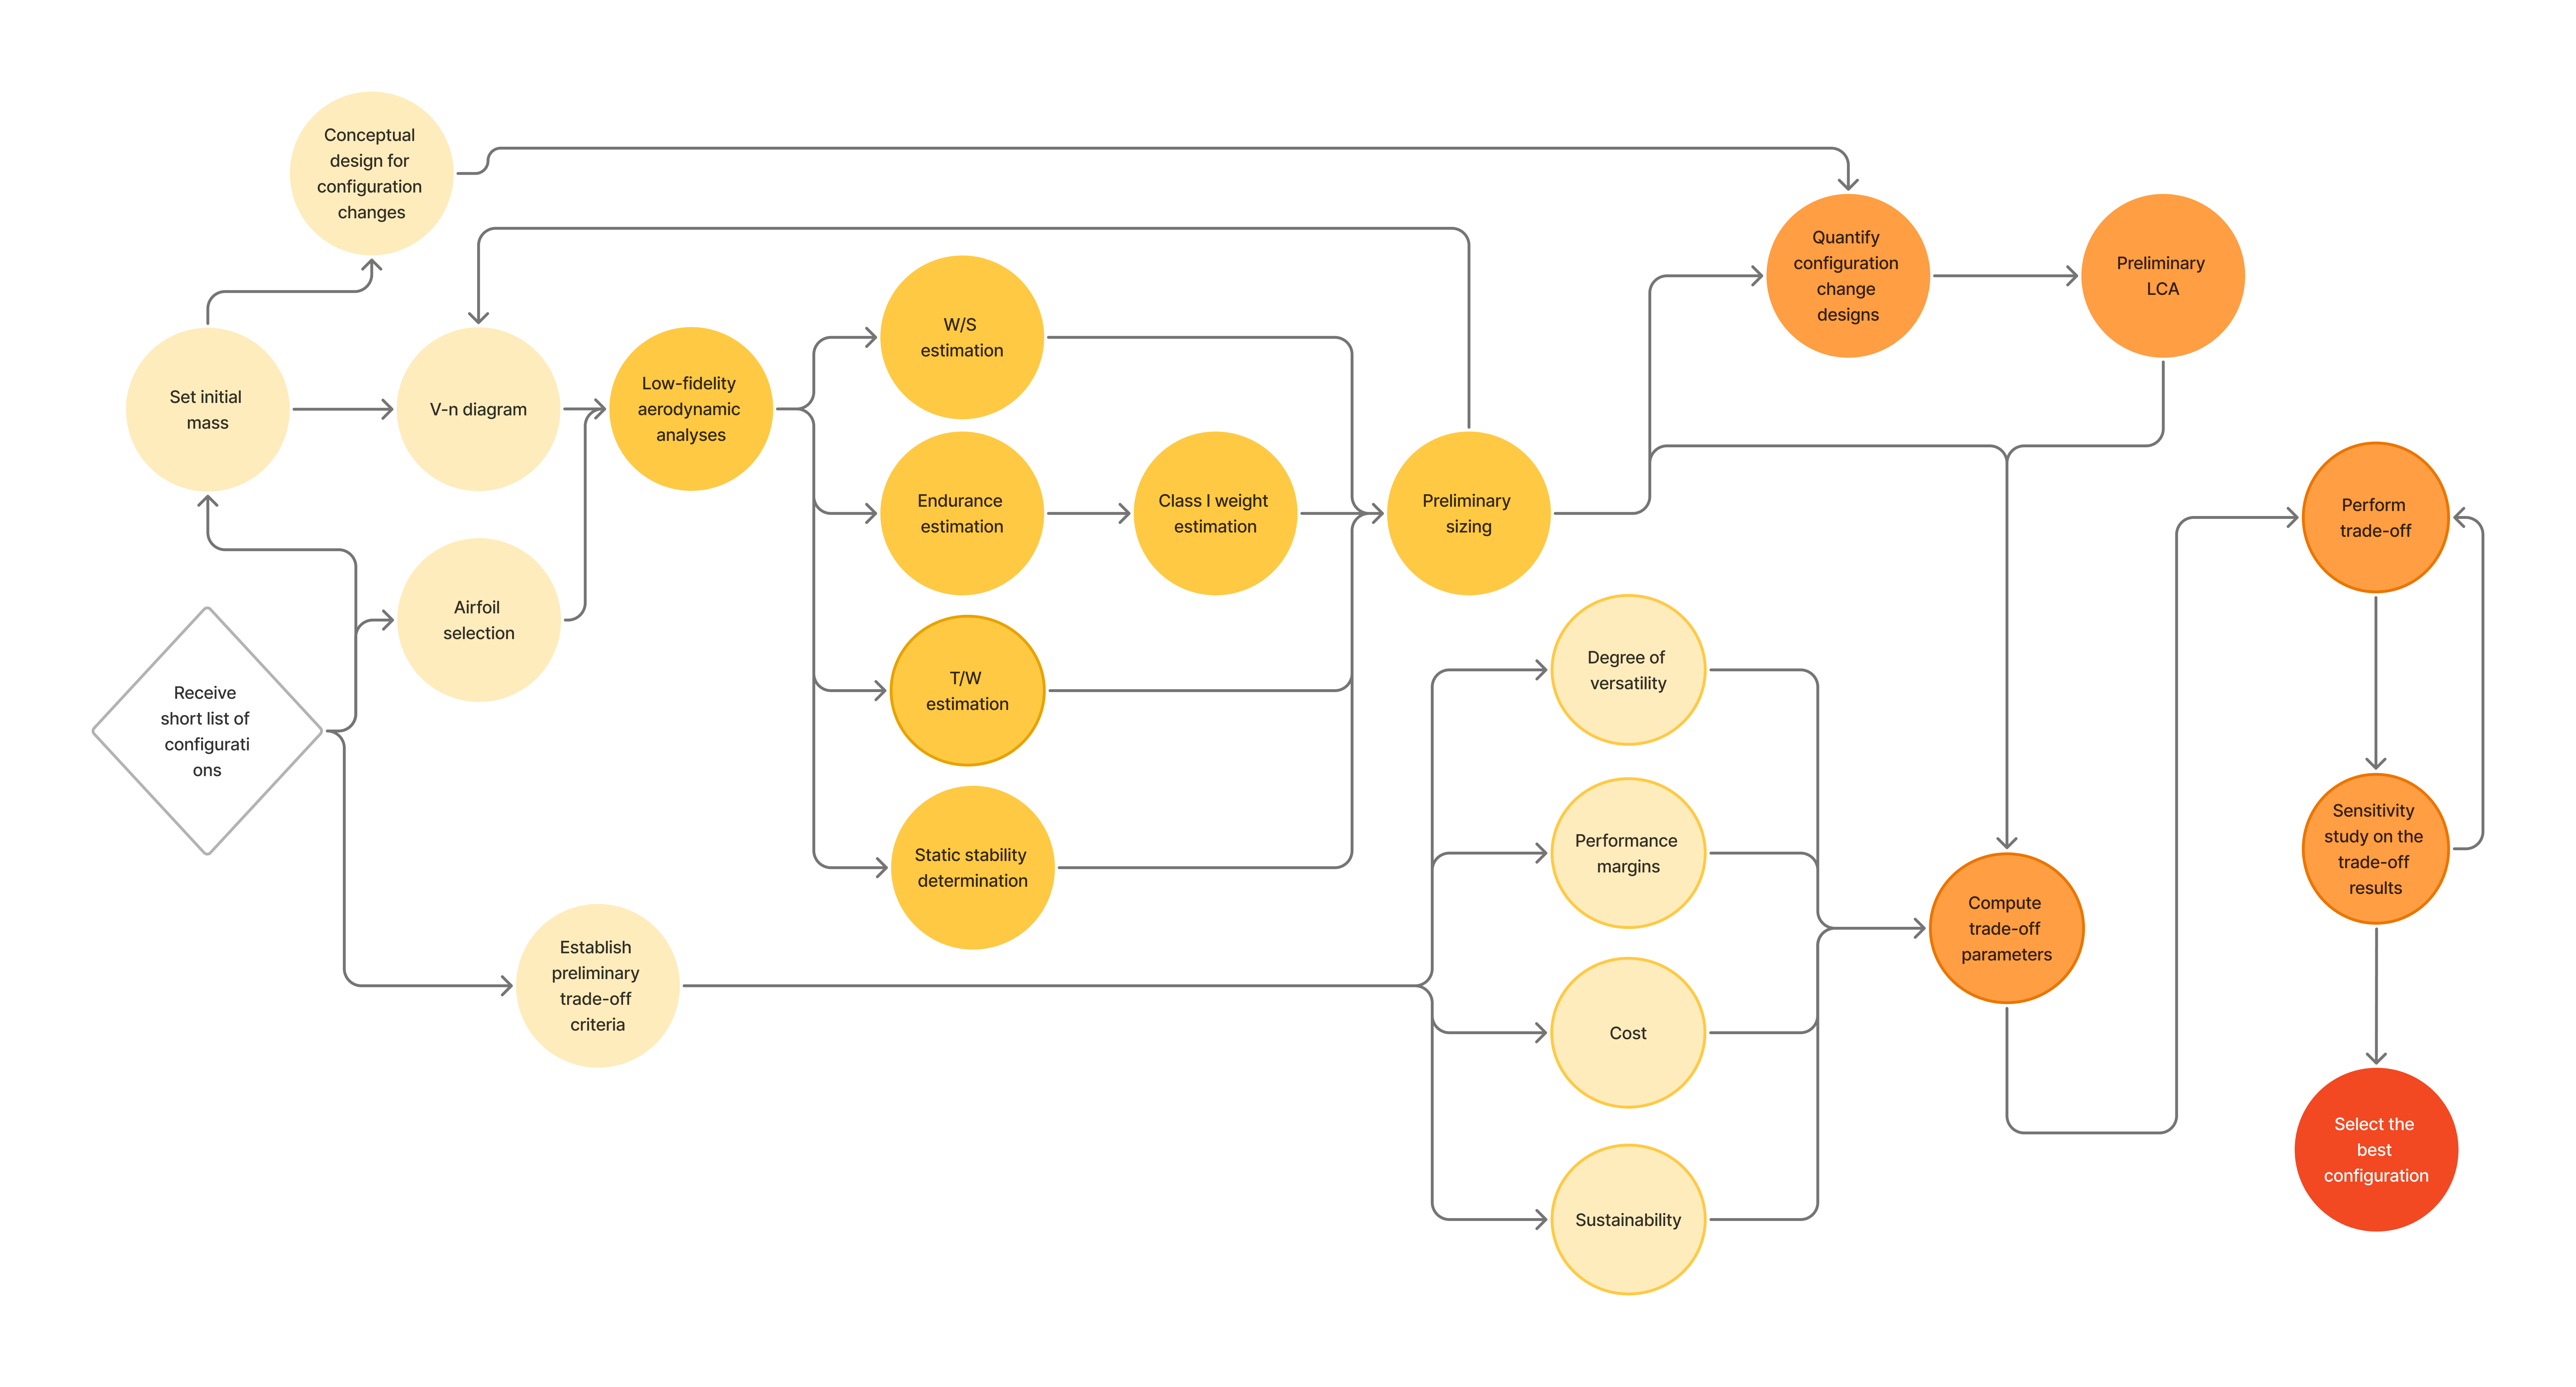
\includegraphics[width=1.4\linewidth, angle=90]{figures/Mid-term workflow.jpg}
%     \caption{Midterm Workflow Diagram}
%     \label{fig:workflow_midterm}
% \end{figure}
% \clearpage
% \pdfpagewidth=420mm
% \pdfpageheight=297mm
% \paperwidth=420mm
% \paperheight=297mm
% 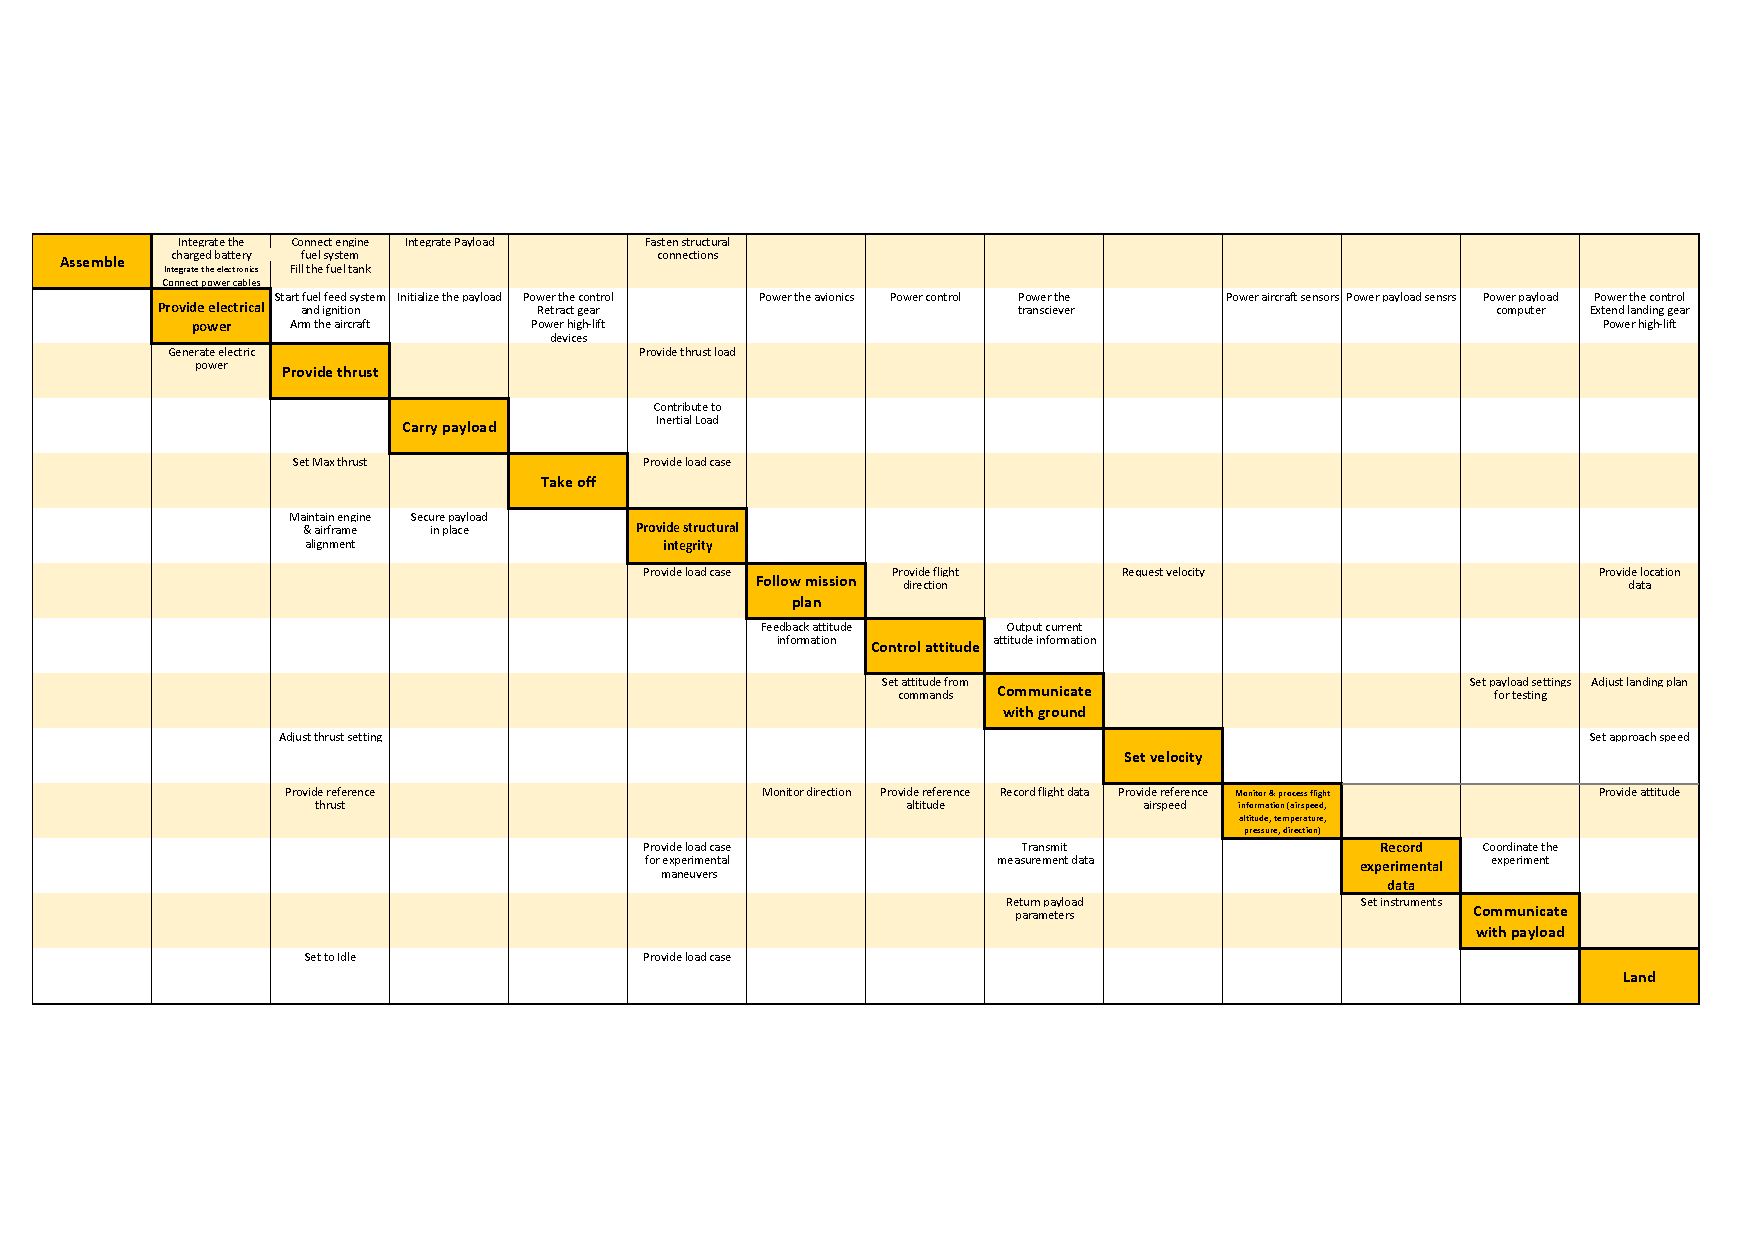
\includepdf[pages=-, fitpaper=true, width=420mm, keepaspectratio, scale=1, pagecommand={
%         \vspace*{\fill} 
%         \thispagestyle{empty} 
%         \noindent\hspace*{0cm} % Adjust this to center the text on the A3 page 
%         \begin{minipage}{400mm} 
%             \captionof{figure}{HUGO platform N2 diagram} 
%             \label{fig: N2}
%         \end{minipage}
%         \vspace*{1.5cm} 
%         \label{fig:N2}
%         % Pushes the caption up from the bottom edge 
%     }]{figures/N2 Diagram.pdf}
% \clearpage
% \pdfpagewidth=210mm
% \pdfpageheight=297mm
% \paperwidth=210mm
% \paperheight=297mm



\section{Project Design \& Development Logic }
\label{sec:Project Design Development Logic}
It is important to keep an outlook for the future of the project and the subsequent development of the aircraft after the design has been completed. To create a more comprehensible diagram, the project design and development were broken down into five different phases \cite{Spitz2001}: 

\begin{enumerate}
    \item \textbf{Development: } Take the preliminary design as input and evaluate the viability of the design. If it is deemed inviable, it is checked whether or not the issues can be solved. If not the project is ended, otherwise the preliminary design is altered until it is viable.   
    \item \textbf{Prototyping and testing:} Each subsystem is designed, manufactured, verified, and validated in isolation. Then, all the subsystems are integrated into a fully functional UAV (Unmanned Aerial Vehicle). The UAV is tested on the ground and in the air to validate the design as a whole.
    \item \textbf{Manufacturing and Certification:} The finalized, validated design is taken into production. In the beginning, the aircraft design is certified by EASA. If it passes certification, the production can begin. If it does not, the design is reiterated. This involves the procurement of off-the-shelf components, and working with manufacturers and suppliers. 
    %for the airframe and other custom components. The final product will then be sent to be certified, along with the required documentation.
    \item \textbf{Operations:} The bulk of the life of an aircraft. Technicians and pilots must be hired and trained. %Operation manuals must be written and procedures must be put into place.Then, the operation certification can be acquired from EASA. 
    HUGO will perform tests required by the client, and undergo necessary design modifications and certification steps requested by the competent authority.
    %the normal operations can begin, including building the aircraft, modifying it to fit the experiment being run by the client, certifying this new configuration if necessary and performing the flight test.
    \item \textbf{End-of-life:} The airframe must be decommissioned responsibly, recycled, or scrapped. The useful components, such as the avionics and actuators, can be repurposed. All other parts must be recycled or disposed of.%if recycling is not possible.
\end{enumerate}
The Project Design \& Development Logic diagram can be seen in \autoref{fig:proj_design} in \autoref{app:project_planning_diagrams}.

\section{Team Organogram \& HR Allocation}
\label{sec:organogram}

To optimise technical development, the team identified and distributed critical organisational responsibilities, as shown in \autoref{fig:organogram} in \autoref{app:project_planning_diagrams}. These roles structure the development process, mitigating internal risks and enhancing the overall quality of the final product. The designated roles and their core functions are as follows:

\begin{itemize}
    \item \textbf{Chairman:} Leads meetings and discussions, prepares agendas, and ensures alignment with team goals.
    \item \textbf{Secretary:} Documents meetings, acts as the primary point of contact for all external stakeholders.
    \item \textbf{Project Manager:} Maintains the project schedule, ensures timely progression and keeps track of deadlines.
    \item \textbf{Chief Systems Engineer:} Oversees technical architecture, ensures integration of the final system.
    \item \textbf{Documentation:} Documentation Manager, Git Manager, and CAD Manager are responsible for managing all text, code, and CAD files. They enforce relevant standards and implement efficient organisation for their respective file types.
    \item \textbf{Sustainability Manager:} Guides the project towards social, economic, and environmental sustainability.
    %sustainable alternatives, ensuring the team operates with ecological responsibility.
    \item \textbf{Quality Assurance Manager:} Ensures all work products meet the standards required by external stakeholders and internal protocols.
\end{itemize}

Additional technical roles were defined to create focused engineering design departments. Each team member was assigned one organisational role and one technical role, and backup members were appointed for each department (names written in bold and italics). Additional members expected to contribute to a specific department were highlighted as "Contributors". The complete Team Organogram is shown in \autoref{fig:organogram} in \autoref{app:project_planning_diagrams}.


%According to the aircraft subsystems described in the Design Option Tree of the Baseline Report \footref{url:baseline_report}, engineering departments were developed and are presented in \autoref{fig:organogram}. Each team member has been assigned as main responsible for a single technical department. Each department has a backup member to become responsible in the case Risk[Team Member absence] were to occur, with their names marked in bold and italics. Other members expected to make significant contributions are named as "Contributors".


\section{Gantt Chart}
\label{sec:planning_gantt_chart}

\autoref{fig:gantt_chart} shows the project Gantt chart outlining the project tasks, along with relevant dependencies and a preliminary timeline.

\begin{figure}[H]
    \centering
    
\includegraphics[width=\linewidth]{figures/GantChart.pdf}
    \caption{Project HUGO Gantt Chart}
    \label{fig:gantt_chart}
\end{figure}